\chapter{EXPERIMENTAL METHODOLOGY AND SETUP}

\section{EVALUATION METHODOLOGY AND STRATEGY}
A central principle of this research is empirical honesty: claims regarding network protocol performance must be established through physical measurement of real network packets rather than theoretical speculation or ungrounded simulations. To achieve both realism and comparative breadth, our evaluation is organized across three complementary tiers:

\begin{figure}[htbp]
    \centering
    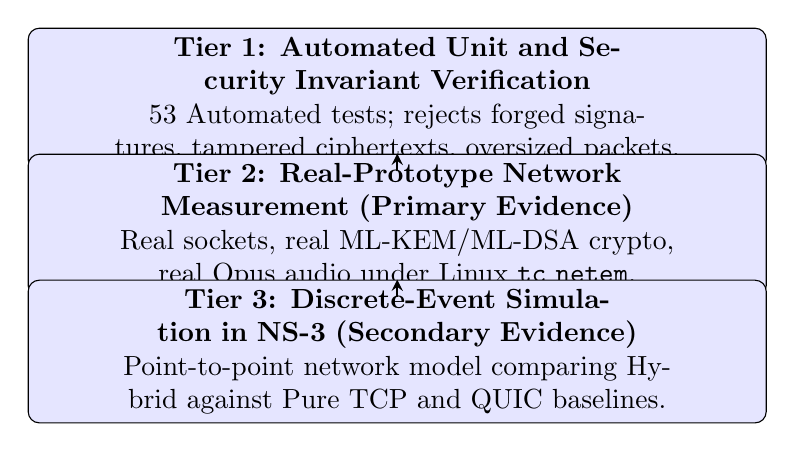
\begin{tikzpicture}[
        every node/.style={align=center},
        tier/.style={rectangle, draw, fill=blue!10, text width=26em, align=center, rounded corners, minimum height=3em},
        conn/.style={thick, ->, >=stealth}
    ]
        \node [tier] (l1) at (0, 3.2) {\textbf{Tier 1: Automated Unit and Security Invariant Verification}\\53 Automated tests; rejects forged signatures, tampered ciphertexts, oversized packets.};
        \node [tier] (l2) at (0, 1.6) {\textbf{Tier 2: Real-Prototype Network Measurement (Primary Evidence)}\\Real sockets, real ML-KEM/ML-DSA crypto, real Opus audio under Linux \texttt{tc netem}.};
        \node [tier] (l3) at (0, 0.0) {\textbf{Tier 3: Discrete-Event Simulation in NS-3 (Secondary Evidence)}\\Point-to-point network model comparing Hybrid against Pure TCP and QUIC baselines.};

        \draw [conn] (l1) -- (l2);
        \draw [conn] (l2) -- (l3);
    \end{tikzpicture}
    \caption{Three-Tiered Evaluation Hierarchy of the HPQV Protocol.}
    \label{fig:evaluation_tiers}
\end{figure}

As documented in Architecture Decision Record 0001 (ADR-0001), the real userspace prototype under Linux Traffic Control (\texttt{tc netem}) serves as the \textbf{primary empirical evidence}. This architectural decision was governed by three physical factors:
\begin{enumerate}
    \item \textbf{Absence of Native PQC in Simulators:} Network simulators such as NS-3 cannot execute cryptographic libraries natively without legacy extensions (such as Direct Code Execution), which are unmaintained and fragile.
    \item \textbf{Realistic Codec and Perceptual Processing:} Simulators treat media as synthetic fixed-rate bit streams. Evaluating speech intelligibility requires running the actual Opus encoder, decoder, and in-band forward error correction routines over real PCM audio.
    \item \textbf{Physical IP Fragmentation Semantics:} Proving that a transport is fragmentation-free requires observing the operating system's IP layer—specifically verifying the absence of IP header More-Fragments (MF) flags and non-zero fragment offsets in raw packet captures.
\end{enumerate}

Simultaneously, as documented in ADR-0003, NS-3 was incorporated as a \textbf{secondary, corroborating model}. NS-3 allows evaluating wide-area propagation delays and benchmarking against protocols (such as QUIC) that cannot be easily embedded into the Python prototype.

\section{REPRODUCIBLE CONTAINERIZED TESTBED}
Linux kernel traffic control (\texttt{tc netem}) and NS-3 do not execute natively on macOS or bare-metal Windows environments. To ensure absolute reproducibility, the complete evaluation suite is packaged within an isolated Ubuntu 24.04 Docker container (\texttt{eval/Dockerfile}) equipped with Python 3.11, \texttt{liboqs}, \texttt{libopus}, \texttt{iproute2}, \texttt{tshark}, and NS-3 version 3.41.

\subsection{The Critical Loopback MTU Discovery}
During early experimentation, a perplexing empirical anomaly was discovered: when running oversized naive UDP handshakes inside Docker containers, packet captures reported zero IP fragments, falsely suggesting that fragmentation was not occurring.

Investigation into container network namespaces revealed that Docker's default loopback interface (\texttt{lo}) is configured with an MTU of \textbf{65,536 bytes} ($64\text{ KB}$). Under a 64 KB MTU, a 10,842-byte handshake datagram fits easily within a single unfragmented frame. Without correcting this parameter, any comparison of IP fragmentation silently measures nothing.

To eliminate this artifact, every evaluation runner within our harness explicitly pins the loopback MTU to the standard Ethernet threshold of 1,500 bytes prior to benchmarking, restoring standard configuration upon teardown:
\begin{lstlisting}[language=bash]
# Pin loopback MTU to realistic Ethernet link capacity
ip link set dev lo mtu 1500
\end{lstlisting}

\section{TRACK 2: REAL-PROTOTYPE EXPERIMENTAL SETUP}

\subsection{Impairment Injection via Linux Traffic Control}
Impairments are injected directly into the Linux kernel network stack using the \texttt{netem} queuing discipline attached to the root qdisc of the loopback interface:
\begin{lstlisting}[language=bash]
# Example: Inject 20% packet loss with 50 ms delay and 10 ms jitter
tc qdisc add dev lo root netem delay 50ms 10ms loss 20%
\end{lstlisting}
Two systematic experimental sweeps were executed:
\begin{enumerate}
    \item \textbf{Loss Sweep:} Packet loss evaluated across $p \in \{0\%, 5\%, 10\%, 20\%, 30\%\}$, with round-trip delay fixed at 50 ms and jitter at 10 ms. Each condition is measured across 5 independent runs, with the median value reported.
    \item \textbf{Latency Sweep:} Propagation delay evaluated across round-trip delays $d \in \{20\text{ ms}, 50\text{ ms}, 100\text{ ms}, 200\text{ ms}\}$ at 0\% loss.
\end{enumerate}

\subsection{Evaluated Protocol Configurations}
Three distinct transport architectures were implemented and benchmarked under identical network conditions:
\begin{itemize}
    \item \textbf{\texttt{hybrid} (Proposed):} HPQV architecture. PQC handshake, mutual authentication, and call signaling run over TCP with 4-byte record framing. Real-time audio streams over UDP with an 11-byte header, ChaCha20-Poly1305 encryption, 1,200-byte cap, and the IP Don't-Fragment bit asserted.
    \item \textbf{\texttt{naive} (UDP Baseline):} Transmits the post-quantum handshake as an oversized UDP datagram without application-level framing, followed by UDP voice streaming. This models how conventional VoIP protocols behave if classical crypto is naively swapped for PQC.
    \item \textbf{\texttt{tcp} (Pure TCP Baseline):} Transmits both the post-quantum handshake and continuous Opus voice frames over a single, persistent TCP connection.
\end{itemize}

\subsection{Telemetry and Packet Capture Instrumentation}
During each benchmark run, a background instance of \texttt{tshark} captures all loopback traffic into a standard PCAP file. IP fragments are detected and quantified using the exact Wireshark display filter:
\begin{lstlisting}[language=bash]
tshark -r capture.pcap \
  -Y "ip.flags.mf == 1 || ip.frag_offset > 0" | wc -l
\end{lstlisting}

\section{TRACK 3: NS-3 DISCRETE-EVENT SIMULATION SETUP}

\subsection{Simulation Topology and Parameter Calibration}
The secondary simulation is implemented in \texttt{ns3/hpqv\_sim.cc}. Two nodes are interconnected via a point-to-point link configured with 10 Mbps bandwidth and a configurable one-way delay ($\text{delay} = \text{delayMs}/2$). A \texttt{RateErrorModel} attached to the receiver randomly drops packets according to the configured loss percentage.

\begin{figure}[htbp]
    \centering
    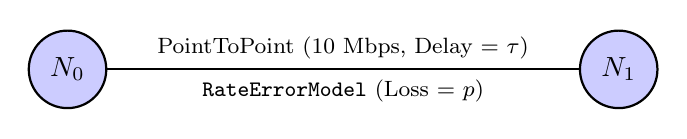
\begin{tikzpicture}[
        every node/.style={align=center},
        nsnode/.style={circle, draw, fill=blue!20, thick, minimum size=2.8em},
        conn/.style={thick}
    ]
        \node [nsnode] (n0) at (-3.5, 0) {$N_0$};
        \node [nsnode] (n1) at (3.5, 0) {$N_1$};

        \draw [conn] (n0) -- node[above]{\footnotesize PointToPoint (10 Mbps, Delay = $\tau$)} 
                            node[below]{\footnotesize \texttt{RateErrorModel} (Loss = $p$)} (n1);
    \end{tikzpicture}
    \caption{NS-3 Point-to-Point Evaluation Topology.}
    \label{fig:ns3_topology}
\end{figure}

The simulation accurately calibrates post-quantum overhead without running crypto:
\begin{itemize}
    \item \textbf{Handshake Volume:} The handshake is modeled as a transfer of exactly 10,842 bytes.
    \item \textbf{Handshake CPU Delay:} A real CPU execution latency of 0.34 ms (derived from benchmarking \texttt{liboqs} on an x86\_64 processor) is injected as an initial application-level scheduling offset.
    \item \textbf{Voice Traffic:} Modeled as a Constant Bit Rate (CBR) stream generating 20 ms frames matching Opus packet sizes.
\end{itemize}

\subsection{Simulation Baseline Schemes}
\begin{itemize}
    \item \textbf{\texttt{hybrid}:} TCP connection for 10,842-byte handshake followed by UDP voice.
    \item \textbf{\texttt{tcp}:} Full TCP transport carrying both handshake and voice stream.
    \item \textbf{\texttt{quic}:} Approximates QUIC by executing a 1-RTT UDP burst handshake (10,842 bytes) followed by UDP voice streaming.
\end{itemize}

\subsection{Documented Limitations of the Simulation Model}
In accordance with academic rigor, three known limitations of the NS-3 model are explicitly documented:
\begin{enumerate}
    \item \textbf{QUIC is a Proxy:} NS-3 3.41 lacks an official, standardized QUIC module. The QUIC baseline models a 1-RTT UDP handshake burst; it does not model QUIC's congestion control or flow control states.
    \item \textbf{Understated TCP Head-of-Line Blocking:} In NS-3, \texttt{FlowMonitor} timestamps each retransmitted TCP segment as an independent fresh packet upon arrival. Consequently, delivery delay for retransmitted frames is understated, causing TCP voice MOS in NS-3 to appear artificially high under heavy packet loss. In reality, head-of-line blocking stalls playback buffers.
    \item \textbf{Zero Queueing Jitter:} Because the simulation models an isolated single flow across an uncontended point-to-point link, queueing variance is negligible. Real-world jitter is captured in Track 2 measurements.
\end{enumerate}

\section{QUANTITATIVE METRICS AND MATHEMATICAL FORMULATIONS}

\subsection{Fragment Count}
Measures the absolute number of physical IP fragments observed in the packet trace. The design objective of HPQV is strictly:
\begin{equation}
    F_{\text{hybrid}} = 0\quad \forall\ p \in [0, 0.30]
\end{equation}

\subsection{Handshake Survival Probability}
Evaluated across 100 consecutive connection attempts per condition. The empirical success proportion is:
\begin{equation}
    \hat{p}_{\text{success}} = \frac{k}{n} = \frac{\text{Successful Handshakes}}{100}
\end{equation}
Because sample size is finite ($n=100$), we calculate the two-sided \textbf{Wilson Score 95\% Confidence Interval} rather than standard normal approximations, ensuring accurate bounds near 0\% and 100\%:
\begin{equation}
    \text{CI}_{95\%} = \frac{\hat{p} + \frac{z^2}{2n} \pm z \sqrt{\frac{\hat{p}(1-\hat{p})}{n} + \frac{z^2}{4n^2}}}{1 + \frac{z^2}{n}}
\end{equation}
where $z = 1.96$ for the 95\% confidence level.

The empirical results are compared directly against the theoretical fragment-loss decay curve:
\begin{equation}
    P_{\text{theory}}(p) = (1 - p)^8
\end{equation}

\subsection{Time to First Byte (TTFB)}
Measures the duration from the dispatch of the initial connection request until the arrival of the first authenticated voice datagram at the receiver:
\begin{equation}
    \text{TTFB} = t_{\text{first\_voice\_received}} - t_{\text{call\_initiated}}
\end{equation}
TTFB captures TCP 3-way handshake round trips, PQC key encapsulation/decapsulation CPU processing, signature generation/verification, and initial datagram transit.

\subsection{Mean Opinion Score (ITU-T G.107 E-Model)}
Voice quality is evaluated using the standardized ITU-T G.107 computational E-model \cite{itut_g107}. The transmission rating factor $R$ is formulated as:
\begin{equation}
    R = 94.2 - I_d(\text{delay}) - I_{e,\text{eff}}(\text{loss})
\end{equation}
where delay impairment $I_d$ is computed from one-way delay $d$:
\begin{equation}
    I_d = 0.024 d + 0.11 (d - 177.3) \cdot \mathbb{I}(d > 177.3)
\end{equation}
and effective equipment impairment $I_{e,\text{eff}}$ for Opus under packet loss $p$ is modeled as:
\begin{equation}
    I_{e,\text{eff}} = 11 + (95 - 11) \cdot \frac{p}{p + 4.3}
\end{equation}
The rating factor $R$ converts to MOS via Equation (2.6).

\subsection{Segmental Signal-to-Noise Ratio (SNR) for FEC Recovery}
To assess the physical reconstruction fidelity of Opus in-band Forward Error Correction (LBRR), an isolated acoustic experiment is conducted using a deterministic 200 Hz to 2,000 Hz acoustic chirp sampled at 48 kHz across 20 ms frames ($N = 960$ samples).

\textbf{Methodological Breakthrough in Reference Selection:} 
Opus is a perceptual lossy codec. Even on a perfect, loss-free network, the decoded PCM waveform differs from the original analog input waveform due to psychoacoustic quantization noise. An early prototype compared lossy reconstructions against the raw uncompressed input PCM, which produced negative SNR values at 0\% loss and non-monotonic curves because codec quantization noise masked the packet loss damage.

To isolate packet loss damage from codec compression noise, the reference signal $s(n)$ is defined as the \textbf{undamaged Opus decode of the identical packet stream}. Any measured error is therefore strictly attributable to packet loss and recovery behavior.

For frame $m$ across $M$ frames, segmental SNR is:
\begin{equation}
    \text{SNR}_{\text{seg}} = \frac{1}{M} \sum_{m=0}^{M-1} 10 \log_{10} \left( \frac{\sum_{n=0}^{N-1} s_m^2(n)}{\sum_{n=0}^{N-1} (s_m(n) - \hat{s}_m(n))^2 + \epsilon} \right)
\end{equation}
At 0\% packet loss, the reconstruction is bit-identical to the reference ($\hat{s}_m(n) = s_m(n)$), resulting in an infinite mathematical SNR. To prevent arithmetic overflow and reporting ambiguities, noise-free frames are explicitly capped at \textbf{99.0 dB}.
